% \chapter{实验测试与结果分析}

% \section{实验环境与测试负载}
% \subsection{硬件配置}

% 使用性能较低的笔记本电脑作为实验平台,具体配置如下:
% \begin{table}[h]
%     \centering
%     \begin{tabular}{ll}
%         \toprule
%         CPU & Intel(R) Core(TM) i7-8750H @ 2.20GHz \\
%         \midrule
%         Memory & 16GB (2 × 8GB) DDR4 @ 2667MT/s SODIMM \\
%         \midrule
%         SSD & Intel SSDPEKKW256G8 NVMe SSD (256GB, PCIe Gen3 x4)  \\
%         \midrule
%         HDD & Seagate ST1000LM035 HDD (1TB, 5400 RPM) \\
%         \bottomrule
%     \end{tabular}
% \end{table}


% % \begin{itemize}
% %     \item Intel(R) Core(TM) i7-8750H CPU @ 2.20GHz
% %     \item Memory: 16GB (2 × 8GB) DDR4 @ 2667MT/s SODIMM
% %     \item SSD: Intel SSDPEKKW256G8 NVMe SSD (256GB, PCIe Gen3 x4) 
% %     \item HDD:Seagate ST1000LM035 HDD (1TB, 5400 RPM)
% % \end{table}


% 由于硬件限制,实验配置了三种卸载后端,分别是机械磁盘,SSD和zram。主要是由于内核中没有实现官方的rdma 和 nvm的卸载后端。

% 为了能够体现出算法的自适应性,我们决定将zram作为性能最好的卸载后端,所以在测试中,我们使用压缩比非常高的数据来体现

% % \subsection{测试负载}

% % 我们将使用一个web server 这种文件密集型和redis这种内存密集型负载来测试我们算法的有效性。

% % web server 包含主动限流功能,当发生延迟的时候,web server 会主动限流,保证延迟的稳定性,这样的话我们可以用每秒的请求数来衡量web server 这种吞吐量来衡量性能。

% % redis,我们禁止了所有持久化功能,并且关闭了淘汰策略的,因为这些功能策略会有复杂的用户态内存管理,他直接在用户态管理内存,导致我们很难模拟出内存压力。

% % 没有使用数据库这种IO密集型负载,是因为数据库中一半有复杂的用户态内存管理,他们直接在用户态管理内存,并不能体现出我们算法的有效性。

% \section{模块功能与有效性测试}

% \subsection{内存压力模块有效性验证}
% 本节中我们将进行内存压力模块有效性验证,验证我们内存压力模块是否能够正确地模拟内存压力。

% 在测试中,我们使用web server用作测试负载,然后在内核中配置不同的卸载后端,然后通过mpfs查看内核是否量化了内存压力。我们多次测试,从16GB一直到6GB,发现10GB是一个临界值,10GB系统不至于崩溃但是性能开始下降了。

% 对于web server ,它包含大量的高清图片和文字,有很高的压缩比。压力发生器就是纯随机的向发送请求,里面包含大量的字符以及高清图片。
% web server 中的包含限速模块,一旦发生延迟,就会主动限速,保证延迟的稳定性。

% \begin{figure}[h]
%     \centering
%     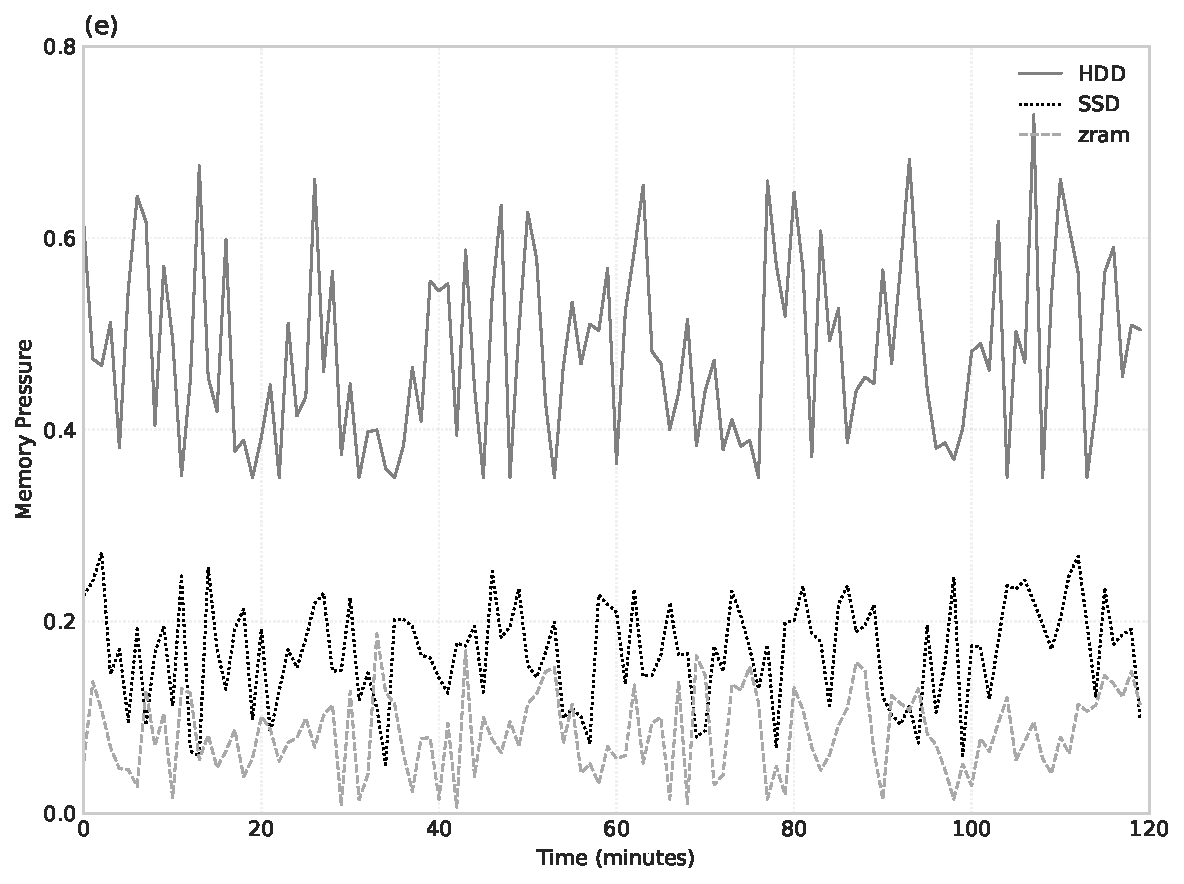
\includegraphics[width=\textwidth]{memory_pressure.pdf}
%     \caption{不同后端的内存压力}
%     \label{fig:memory_pressure}
% \end{figure}

% 如图\ref{fig:memory_pressure}所示,我们测试了三种不同的卸载后端,分别是机械硬盘,SSD和zram,横轴时时间,纵轴是内存压力。

% 同样的负载,内核感知到了不同的内存压力,机械硬盘的内存压力最大,有一半的时间用来换入换出,系统基本无法正常响应。ssd和zram的内存压力比较较小,系统可以正常工作。



% \subsection{文件页与匿名页均衡算法有效性验证}

% 我们选用了10GB的内存,然后使用web server 作为测试负载,然后使用压力发生器来模拟内存压力。

% 我们改动swappiness 从 0 60 100 ,测试了不同的swappiness 对系统性能的影响。
% 然后我们ebpf程序来hook函数,查看内核的refault次数。
% 由于是文件页面和匿名页面,所以选择了文件密集型的web server 以及内存密集型的redis作为负载,其中redis禁止了所有持久化功能,并且关闭了淘汰策略的,因为这些功能策略会有复杂的用户态内存管理,他直接在用户态管理内存,导致我们很难模拟出内存压力。


%     我们首先测试了默认情况下不同的swappinness,web server 的性能表现。
    
%     结果如图\ref{fig:web_server_swappiness}所示:
%     \begin{figure}[h]
%         \centering
%         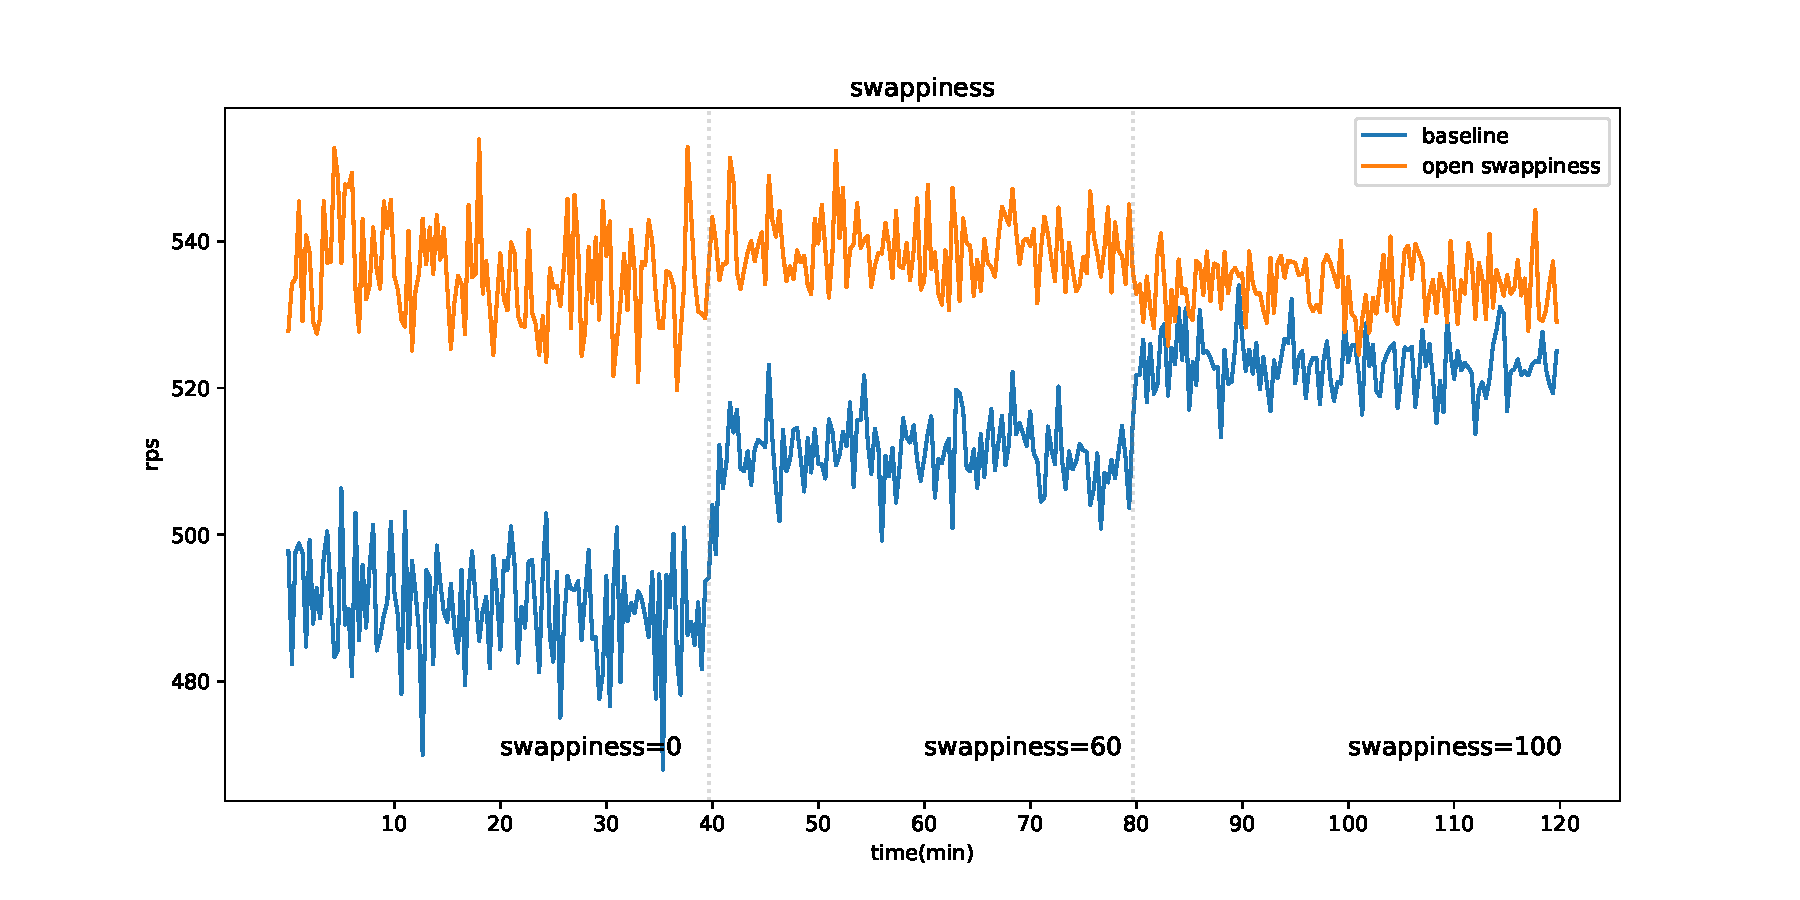
\includegraphics[width=\textwidth]{swappiness.pdf}
%         \caption{web server 的swappiness 性能}
%         \label{fig:web_server_swappiness}
%     \end{figure}

%     可以swappiness 为0的时候,由于过度回收文件页,性能是最差的。
%     随着swappiness 的增加,性能逐步提升。因为内核开始回收匿名页,缓解了文件页的压力。

%     现在测试开启了我们的算法,结果如下:

%     无论swappiness 为多少,我们的算法都能够保证性能的稳定,甚至还能进一步加强对匿名页码的回收,提升web server的性能。



%     对于redis,由于是内存密集型,
%     \begin{table}[h]
%         \centering
%         \begin{tabular}{cc}
%             \toprule
%             swappiness & 平均rps \\
%             \midrule  
%             0 & 482 \\
%             60 & 573 \\
%             100 & 540 \\
%             \bottomrule
%         \end{tabular}
%     \end{table}
%     在部分满足的时候,swappiness 为0的时候,倾向于回收文件页,性能并没有很好。
%     并且随着swappiness 的增加,开始倾向于回收匿名页,性能有了略微的提升,
%     这跟我们最初的预想有一定出入,我们最初预想的是随着swappiness 的增加,开始倾向于回收文件页,性能会进一步下降。我们分析了原因,我们使用smaps来分析内存,发现了匿名页和文件页的比例非常夸张,有20:1的比例,所以即使回收文件页面也回收不了多少,并且这些文件页面甚至是对应的程序文件页,造成严重的refault。所以我们回收匿名页,有了空间,性能开始提升了。
%     我们在这种内存密集型负载中,由于文件页确实比较少,导致文件页的refault次数比较少,起不到很好的提交作用,提升性能有限。
%     但是随着swappiness 的增加,开始过多回收匿名页,导致匿名页的refault次数增加,又开始下降了。所以怎么让匿名页也开始自适应,是之后的研究内容。


% \section{综合测试}
% \subsection{测试目标}
% 在上面我们验证了两个主要模块的有效性,本节主要是测试本研究提出的方案在实际场景中的性能,能卸载多少内存,会不会对性能有影响。从多个角度来量化

% \subsection{测试方案}

% 我们使用web server来测试,我们首先将通过一轮请求,将整个文件全部加载到工作集中吗,

% 我们首先使用4.12 内核,在不开启swap,使用ssd作为卸载后端,使用zram作为卸载后端,测试了web server 的性能,以及内存使用。
% 然后使用本研究改进的内核,使用\ref{sec:pressure_based_model}中的方法,来计算容器中的工作集大小,我们将阈值配置成0.1\%,测试内存和性能。
% 初次对比了使用ssd和zram作为卸载后端,他们的p90和缺页中断次数。

% 最后我们测试了容器环境下的内存节省。

% \subsection{测试结果与分析}
% \begin{figure}[h]
%     \centering
%     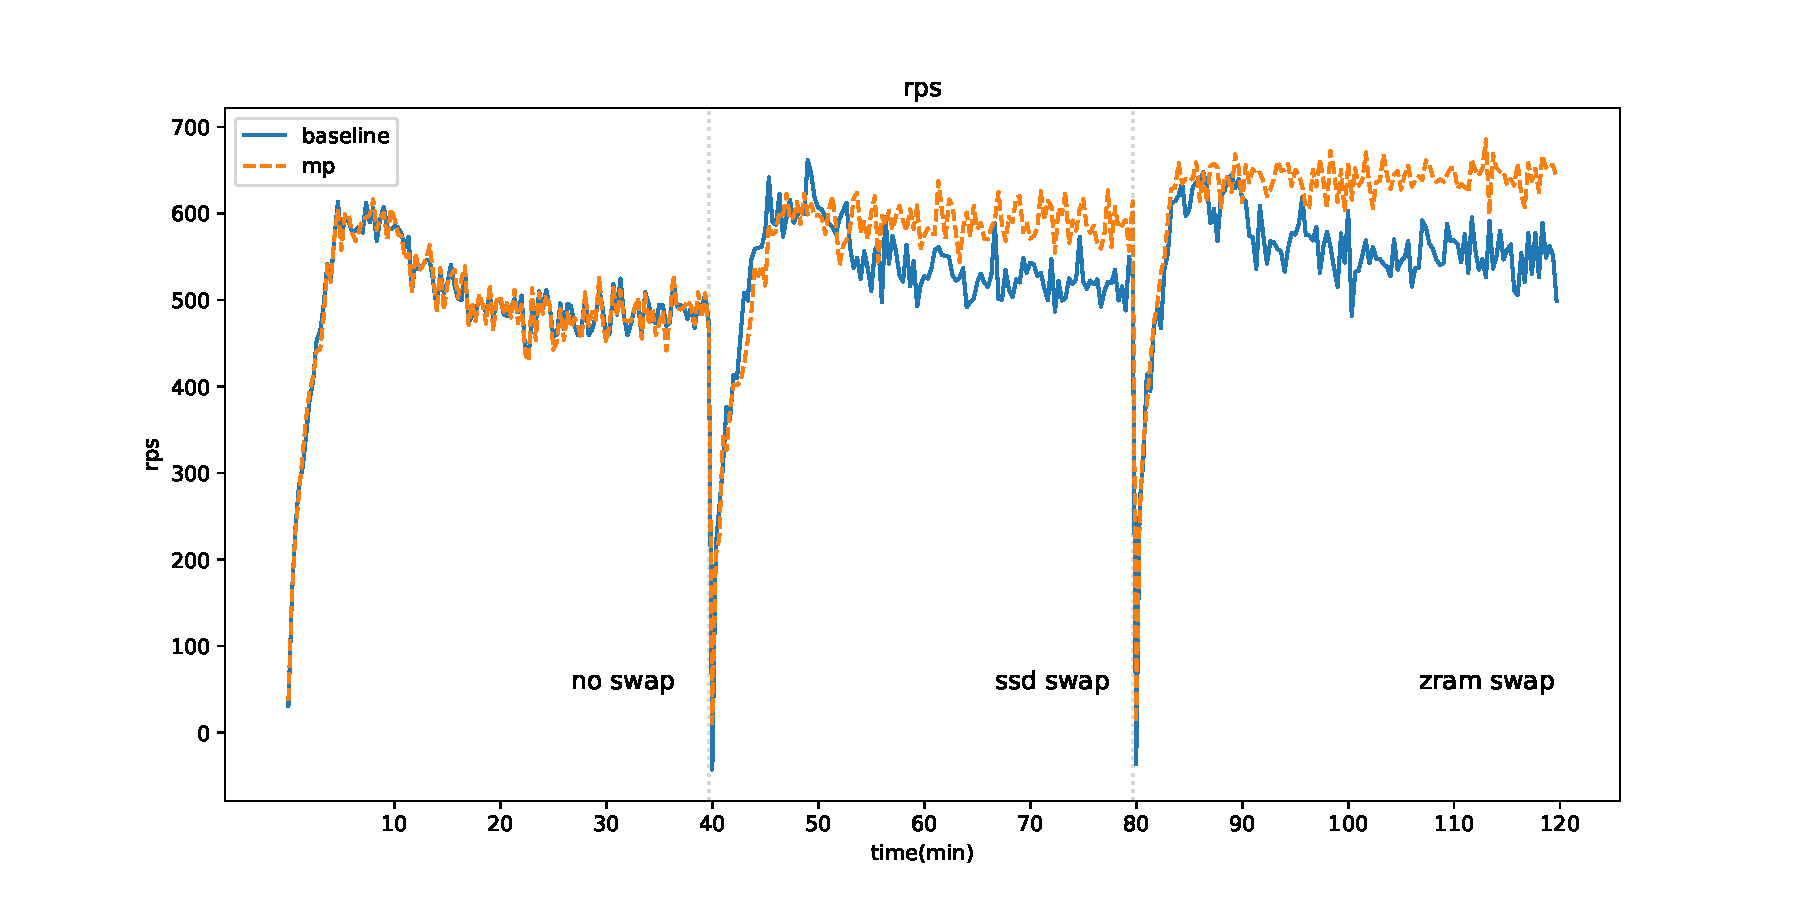
\includegraphics[width=\textwidth]{rps.pdf}
%     \caption{RPS}
%     \label{fig:rps}
% \end{figure}

% \begin{figure}[h]
%     \centering
%     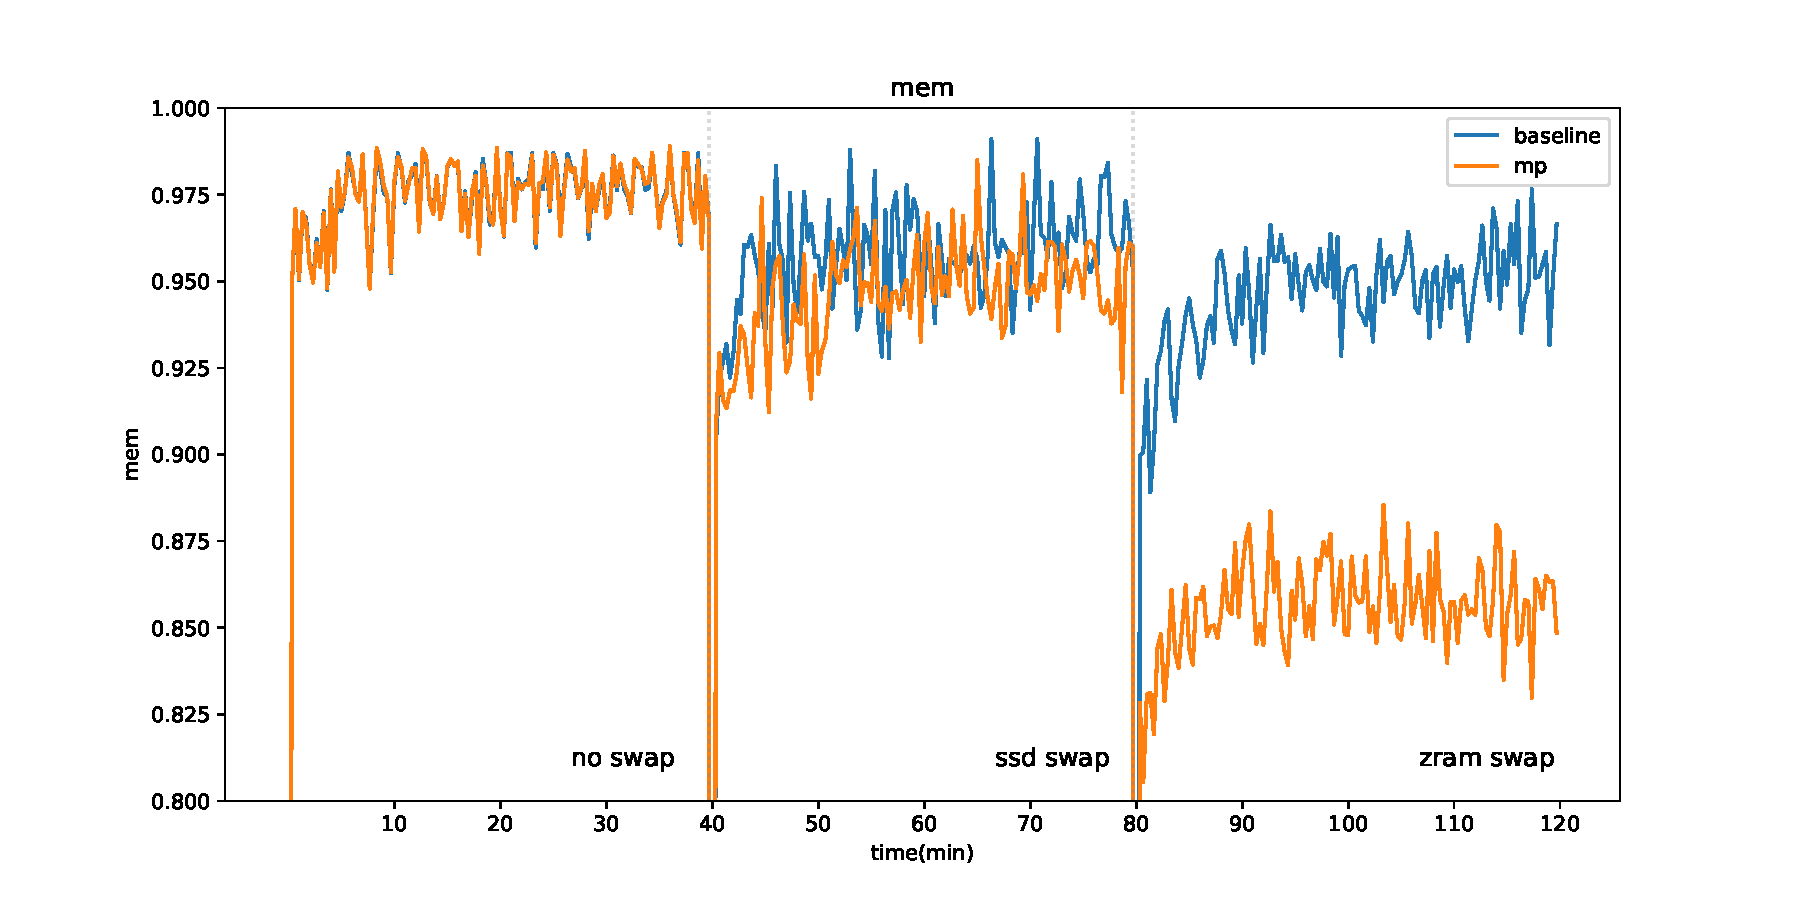
\includegraphics[width=\textwidth]{mem.pdf}
%     \caption{内存使用}
%     \label{fig:mem}
% \end{figure}
% \begin{figure}[h]
%     \centering
%     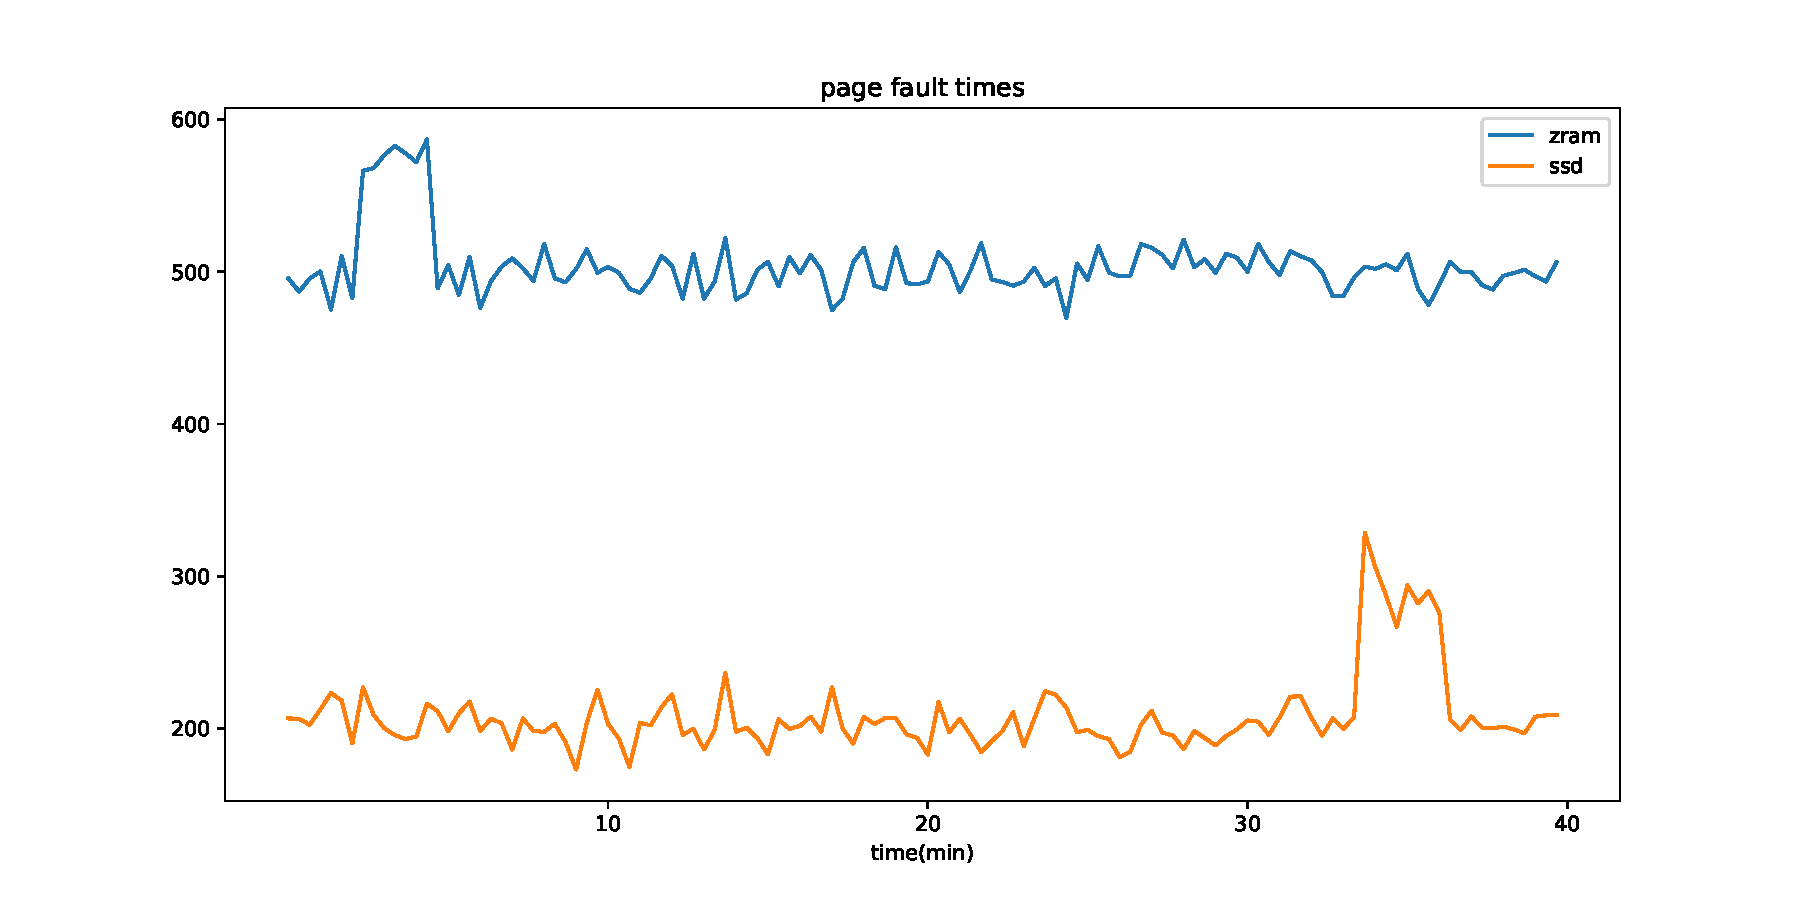
\includegraphics[width=\textwidth]{refault.pdf}
%     \caption{缺页中断次数}
%     \label{fig:refault}
% \end{figure}
% \begin{figure}[h]   
%     \centering
%     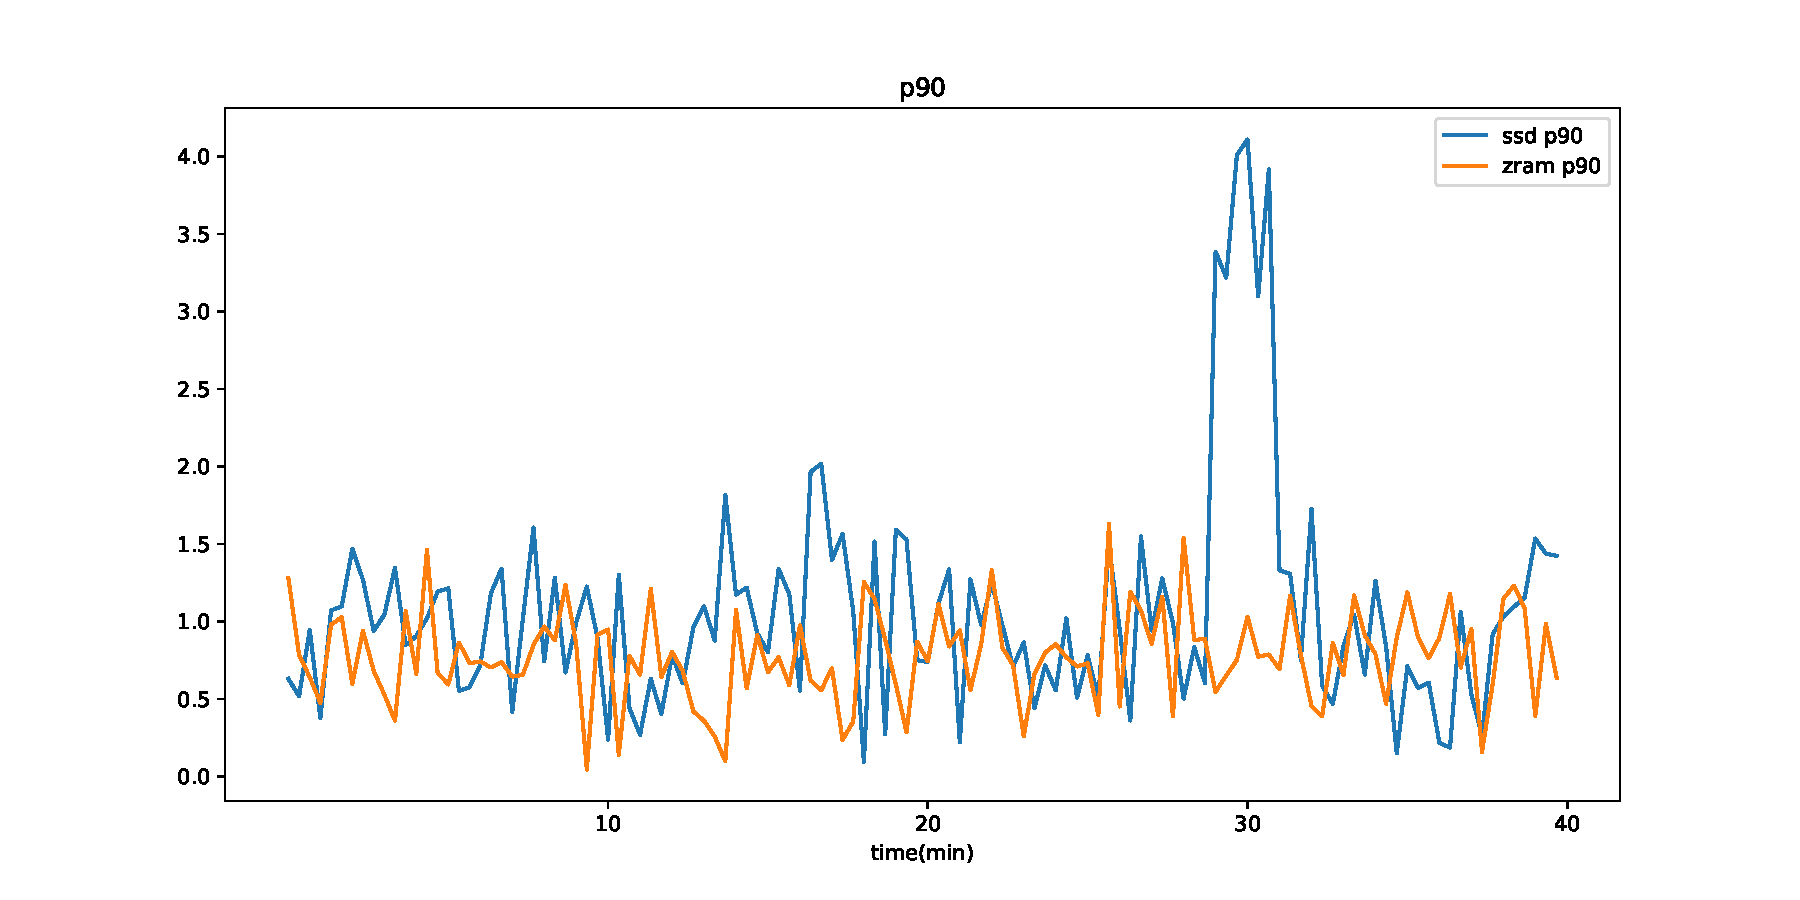
\includegraphics[width=\textwidth]{p90.pdf}
%     \caption{p90 事务响应时间}
%     \label{fig:p90}
% \end{figure}

    
% 本文做了对比实验,一种是开启算法,另一种是不开启。并且分别对比了不开始swap和使用ssd和zram作为卸载后端。

% 如图\ref{fig:rps}所示,我们关注baseline,首先看禁止了swap的时候一开始最高,但是随着不断的处理请求,内存变多,性能下降,导致RPS下降。我们启动了swap,使用ssd作为卸载后端,发现性能有了一些下降,因为开启了这个之后,错误的页面识别导致了错误的页面换入,导致性能下降。zswap同理。

% 我们现在关注使用内存压力,并且不断自适应卸载和调整内存工作集之后,这个rps的表现是比较稳定的,对于ssd来说,基本稳定了性能,对于zram来说,最终的rps也得到了提高。

% 现在我们关注内存使用,如图\ref{fig:mem}所示,如果不开启swap,他的内存使用时固定的,使用了swap,对于ssd来说,他的内存小了,但是没有小太多,zram由于压缩比很高,所以下降的稍微多了一些。

% 现在我们开启了算法,并且使用ssd作为卸载后端,可以看到内存压力进一步下降,但是最明显的还是zram,他的内存压力下降了非常多。节约了内存。

% 现在我们关注缺页中断次数,如图\ref{fig:refault}所示,由于压缩内存内存性能比较高,内核更加积极的进行同步内存回收,所以他的缺页中断次数比较多。

% 现在我们关注p90事务响应时间,如图\ref{fig:p90}所示,可以看到,使用ssd作为卸载后端,由于io性能比较差,所以他的p90事务响应时间比较高,使用zram作为卸载后端,由于io性能比较好,所以他的p90事务响应时间比较低。

% \begin{figure}[h]
%     \centering
%     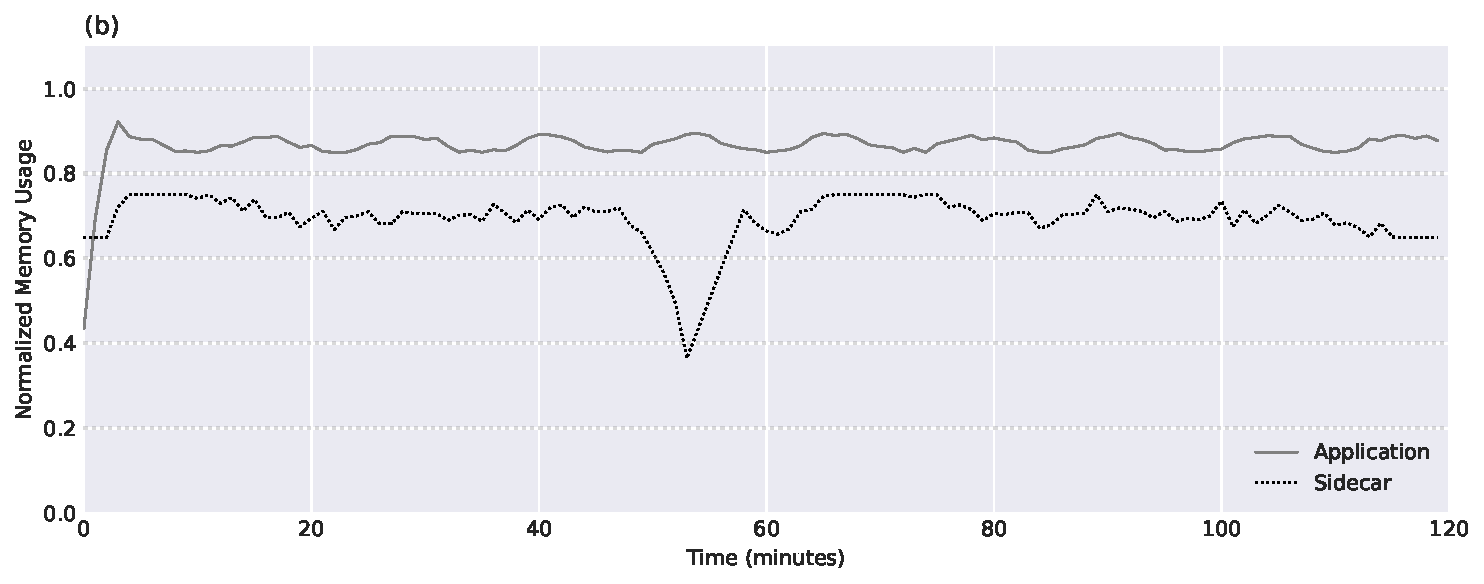
\includegraphics[width=\textwidth]{container_memory.pdf}
%     \caption{容器性能}
%     \label{fig:container_memory}
% \end{figure}

% 下面我们来查看针对虚拟化场景,如图\ref{fig:container_memory}所示,通常,在kubernetes中,我们使用多个pod,Pod 内的每个容器都会有自己独立的 cgroup,但这些容器也会在同一个 Pod 的“父”cgroup(或层级)下。换句话说,Kubernetes 通常会为 Pod 建立一个顶层 cgroup,然后在该 cgroup 下为每个容器创建各自的 cgroup。所以我们为边车容器和负载容器都检测内存压力,然后配置内存大小,发现边车容器和负载容器都得到了内存的释放。边车容器的主要工作就是负责流量的代理转发以及日志的记录,这些操作所占用的资源我们一般成为虚拟化税,随着容器规模的增加,虚拟化税会逐渐增加,导致资源利用率下降。可以看到边车容器的有更大这个内存卸载空间,在大规模的场景下,可以释放更多的内存。



% \section{本章小结}

% 我们验证了内存压力和文件页与匿名页均衡算法在实际场景中的有效性,并且基于内存压力的动态调控模型,可以自适应的调节工作集大小,主动卸载内存,节省了内存。并且我们认为在大规模虚拟化场景下,有大量的pod,其中的边车容器的卸载空间很大,有非常大的卸载空间。


\chapter{实验测试与结果分析}

\section{实验环境与测试负载}

\subsection{硬件配置}

本研究的实验环境选择了一台硬件性能相对有限的笔记本电脑,以更真实地检验内存回收与卸载方案在资源受限场景下的表现。表~\ref{tab:hardware_config}汇总了实验平台的具体配置,可以看到该平台拥有 Intel(R) Core(TM) i7-8750H CPU @ 2.20GHz 以及 16GB DDR4 内存。为了在内核中进行对比,本研究分别选取了机械硬盘、SSD 和 zram 这三种不同的卸载后端。之所以进行这样的选择,一方面是由于官方内核暂未实现基于 RDMA 和 NVM 的卸载后端,另一方面也是为了更好地体现不同存储介质在 I/O 延迟和读写性能方面的差异。机械硬盘能够代表最传统、也是性能相对最差的卸载方式,SSD 在随机读写和延迟方面有一定程度提升,而 zram 则具有数据压缩和低延迟的优势,通常被认为是内存交换的优先方案。为了凸显 zram 的潜在优势,并评估自适应算法在高压缩比数据下的实际效果,本文在后续测试中也将 zram 视为可获得最优 I/O 性能的后端加以重点分析。

\begin{table}[h]
    \centering
    \caption{实验平台硬件配置}
    \label{tab:hardware_config}
    \begin{tabular}{ll}
        \toprule
        CPU & Intel(R) Core(TM) i7-8750H @ 2.20GHz \\
        \midrule
        Memory & 16GB (2 \(\times\) 8GB) DDR4 @ 2667MT/s SODIMM \\
        \midrule
        SSD & Intel SSDPEKKW256G8 NVMe SSD (256GB, PCIe Gen3 x4)  \\
        \midrule
        HDD & Seagate ST1000LM035 HDD (1TB, 5400 RPM) \\
        \bottomrule
    \end{tabular}
\end{table}

在负载选择方面,为了更全面地测试本文提出方案的通用性,实验分别使用了文件密集型的 Web Server 和内存密集型的 Redis 这两类典型应用。Web Server 场景主要用于观察系统针对大量静态文件(包括高清图片与文本数据)缓存时的文件页回收策略,而 Redis 场景则聚焦在匿名页占比极高的内存回收状态。值得注意的是,在 Redis 测试中禁止了持久化功能并关闭了淘汰策略,这样能更直接地暴露内存回收在内核层面的有效性,因为一旦允许用户态自行管理持久化或淘汰,就会在应用层与内核层产生额外耦合,从而干扰对回收策略的评估。

\section{模块功能与有效性测试}

\subsection{内存压力模块有效性验证}

在展开具体算法评估之前,需要首先验证所设计的内存压力模块能否在不借助用户态复杂逻辑的前提下,为系统施加可量化的内存压力。为此,本文使用了 Web Server 作为负载,将各种类型的图片和文字文件提前放入服务器端,随后利用压力发生器随机并持续地发起请求,同时在内核中分别配置机械硬盘、SSD 和 zram 作为卸载后端。通过这样的方式,可以从 16GB 可用内存开始,逐步减少可用空间直到 6GB,借此形成多轮测试,并观察在不同后端介质下系统对内存压力的响应程度。图~\ref{fig:memory_pressure}展示了三种卸载后端下的内存压力曲线。可以明显看出,机械硬盘由于读写延迟和带宽的劣势,会更频繁地陷入换入换出操作,导致系统大量时间都处在高压力区间,甚至难以稳定地对外提供请求服务;相比之下,SSD 提供了更快的 I/O 响应能力,zram 在具有压缩和低访问延迟的双重优势下,则能进一步缓解内存压力飙升的问题。通过该实验可以确认本研究的内存压力模块在不同后端下均能触发与还原高压场景所需的换页流程,且能够准确地量化系统内存使用状况,为后续的自适应回收算法测试奠定基础。

\begin{figure}[h]
    \centering
    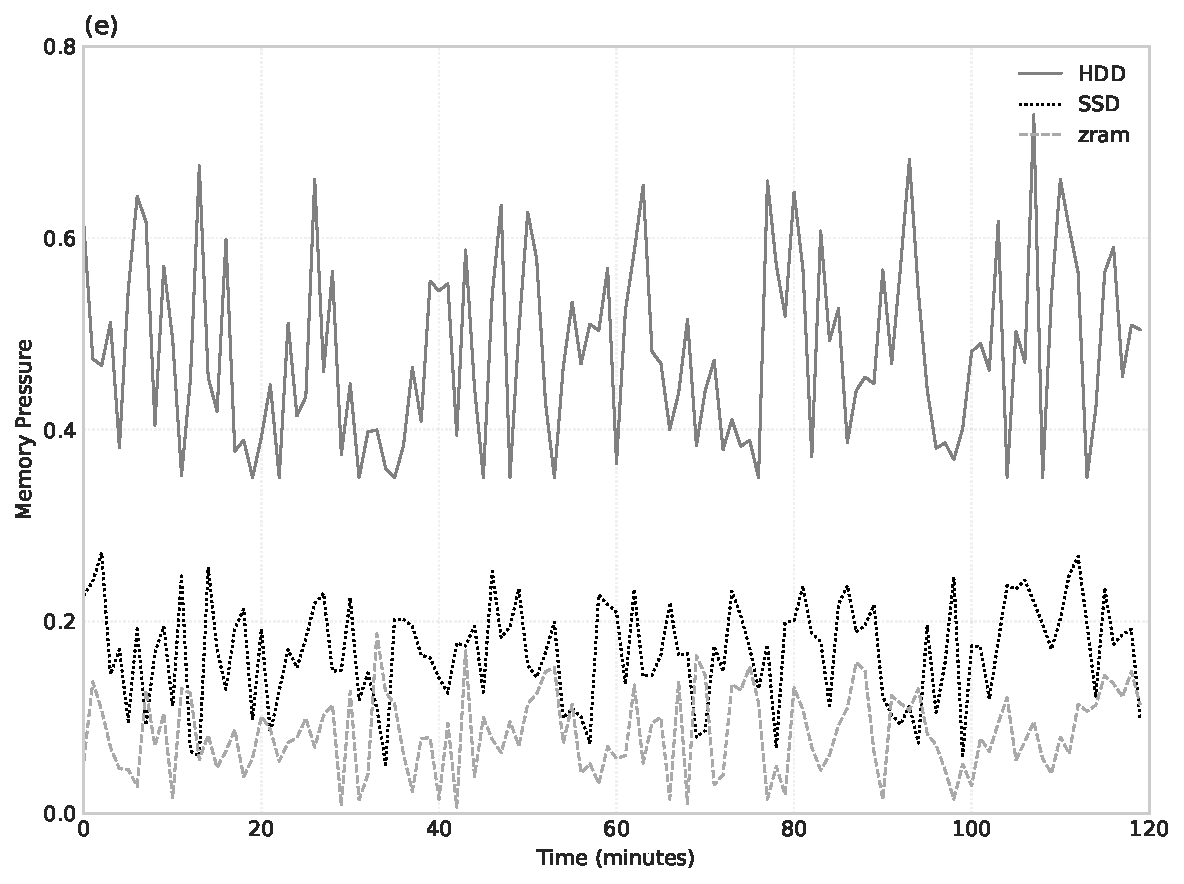
\includegraphics[width=\textwidth]{memory_pressure.pdf}
    \caption{三种卸载后端下的内存压力对比}
    \label{fig:memory_pressure}
\end{figure}

\subsection{文件页与匿名页均衡算法有效性验证}
\label{sec:file_page_anonymous_page_balance_algorithm_validation}

在确认内存压力模块可以生成可控且真实的压力环境后,需要检验自适应回收算法的第二个核心:即针对文件页与匿名页的均衡回收机制。为此,本文选取了 10GB 的可用内存作为上限来运行高负载场景,并针对 Linux 内核中的 \texttt{swappiness} 参数进行多轮对比测试。首先在文件密集型负载(Web Server)下,测试 \texttt{swappiness} 等于 0、60 以及 100 的情况,记录系统在默认内核策略下的吞吐量(RPS)与性能变化,并使用 eBPF Hook 观测关键函数处的 refault 次数。图\ref{fig:web_server_swappiness} 说明了当 \texttt{swappiness}=0 时,内核过度回收了文件页,导致高速缓存不足,Web Server 因频繁的磁盘 I/O 而性能大幅下滑;当 \texttt{swappiness} 提升至 60 或 100 时,系统开始更多回收匿名页,文件页的占用得到缓解,性能有所回升。随后在相同场景下启用自适应均衡算法,结果显示无论 \texttt{swappiness} 处在何种值,该算法都能在文件密集型负载中维持一个相对稳定甚至更高的吞吐,这表明算法能够基于实际页面访问特征,适度地回收匿名页并保留更多活跃的文件页,从而减少了不必要的磁盘 I/O 再加载。

\begin{figure}[h]
    \centering
    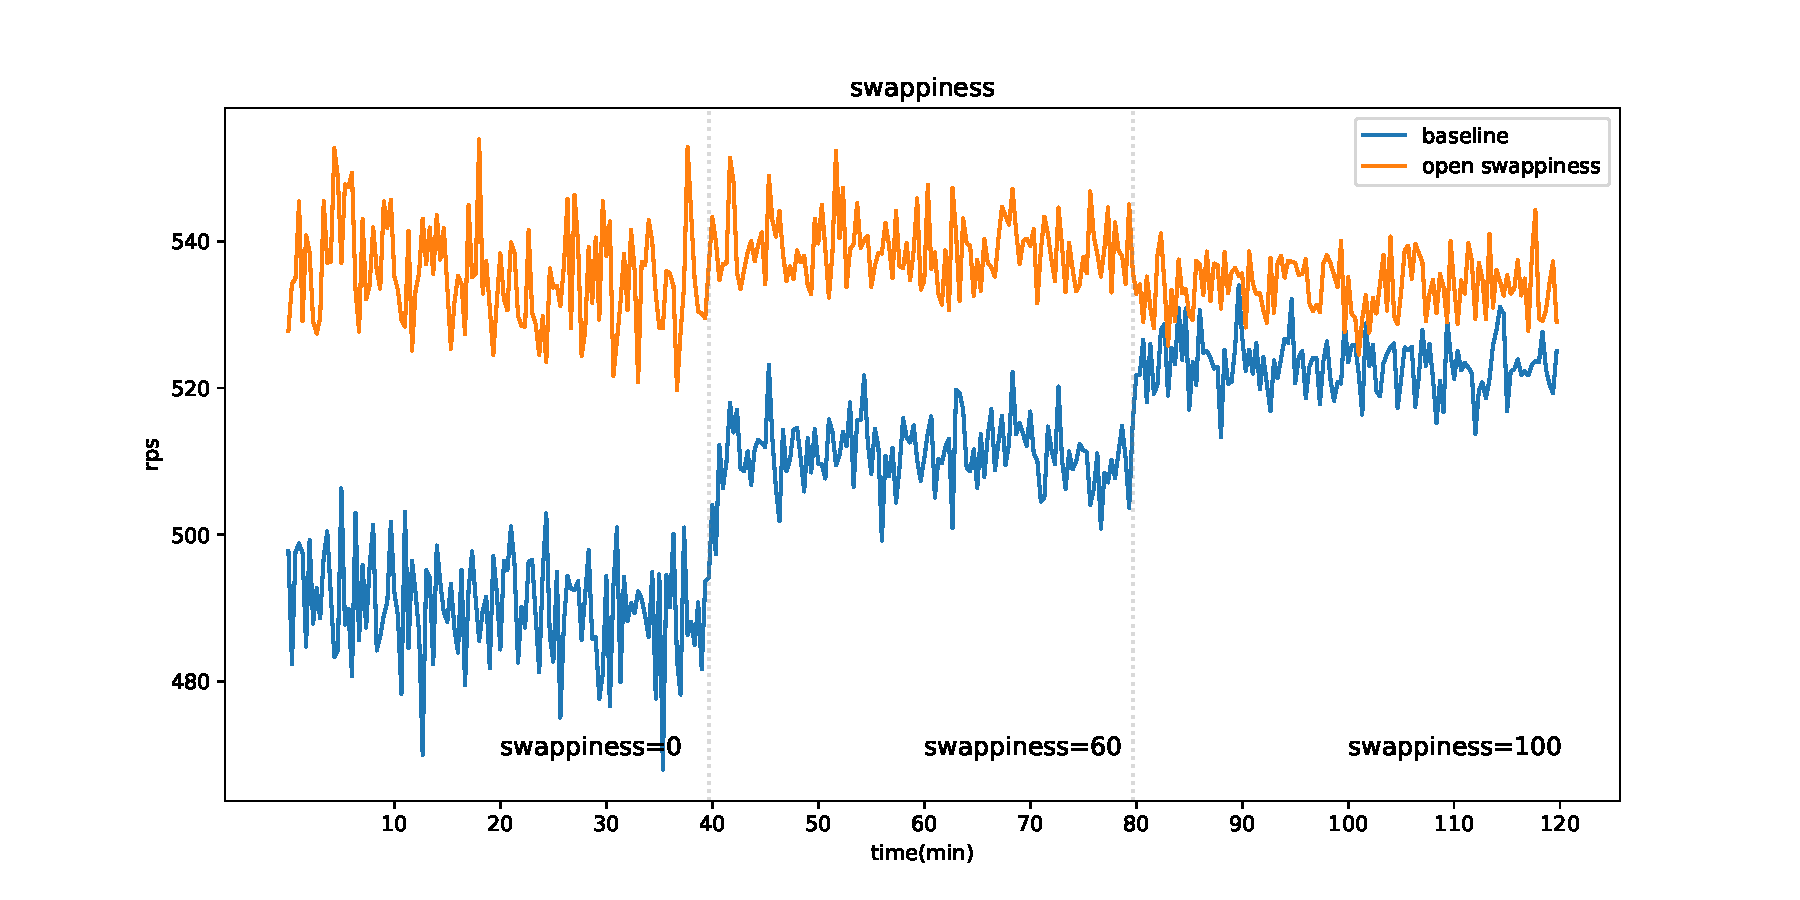
\includegraphics[width=\textwidth]{swappiness.pdf}
    \caption{Web Server 在不同 \texttt{swappiness} 下的性能变化}
    \label{fig:web_server_swappiness}
\end{figure}

    \begin{table}[h]
        \centering
        \label{tab:redis_swappiness}
        \begin{tabular}{cc}
            \toprule
            swappiness & 平均rps \\
            \midrule  
            0 & 482 \\
            60 & 573 \\
            100 & 540 \\
            \bottomrule
        \end{tabular}
    \end{table}

与此同时,为了验证在极高匿名页占比的环境中算法同样适用,本文选取了 Redis 负载作为测试对象,并同样设置了 \texttt{swappiness} 的多档取值。测试结果表明,在 \texttt{swappiness}=0 时,由于基本不回收匿名页,系统受制于内存紧张始终处于高负载状态,平均 RPS 最低;当将 \texttt{swappiness} 提高至 60,系统将更多匿名页移出,使得有空间保留其它必要页面,性能反而有了较大提升;若将 \texttt{swappiness} 增加到 100,回收匿名页变得过于激进,频繁触发缺页中断,导致 RPS 又有所回落。这说明,在匿名页占主导的场景中,适度地回收匿名页能提升整体吞吐,而过度回收则会导致换入换出过于频繁,削弱性能。通过文件密集型和内存密集型两类应用的双重实验,可以初步确认本文提出的文件页与匿名页均衡算法能够在实际环境中奏效,并具有一定的通用价值。

我们测试了redis在不同swappiness下的性能,并同样设置了 \texttt{swappiness} 的多档取值。结果如表~\ref{tab:redis_swappiness}所示。

可以看到测试结果和文件页偏多的web server测试结果有一些偏向,当swappiness=0时,更加偏向于回收文件页,理应性能最高,但是并没有达到预期。我们仔细分析了原因,发现redis的匿名页占比非常高,达到了90\%以上,所以回收匿名页的收益非常小,并且这个时候回收的文件页竟然包含了程序文件。这导致性能比较差。至于swappiness=60和100的时候,开始回收匿名页,60的时候性能更好,100的时候回收了太多的匿名页,性能又开始下降。这个表明我们的算法没有办法自适应的回收匿名页。

\section{综合测试}

\subsection{测试目标}

上述实验对“内存压力模块”以及“文件页与匿名页均衡算法”分别进行了初步验证,证明它们在单项功能上具备有效性。为了更深入地了解将二者结合起来后对系统整体性能和资源使用的影响,本文设计了综合测试。该测试主要聚焦以下问题:在持续提供服务的高负载场景下,若开启自适应算法并在不同后端(SSD 与 zram)进行内存卸载,系统能否稳定提升吞吐量并节约内存占用;在用户态应用(如 Web Server)长期占用大规模文件页以及针对容器化的多进程场景下,算法是否依旧有良好的适应性。

\subsection{测试方案}

首先在 Web Server 场景下,通过一轮预热请求将常见的文件页面基本加载至内存中,以形成完整的工作集,然后维持高并发请求并逐步向系统注入额外的内存压力,依次在以下场景下进行对比:(1) 禁用 \texttt{swap};(2) 启用 \texttt{swap} 并使用 SSD;(3) 启用 \texttt{swap} 并使用 zram;(4) 在(2)与(3)基础上额外启用自适应算法(含内存压力模块、文件页与匿名页均衡及基于压力的工作集评估)。为量化效果,本文重点记录并分析 RPS、系统内存使用量、缺页中断次数(refault)以及 p90 响应时间等关键指标,结合曲线变化对整体性能加以解释。

\subsection{测试结果与分析}
\label{sec:test_result}

图~\ref{fig:rps}~图~\ref{fig:p90}汇总了本研究的主要观测指标,包括系统吞吐量、内存使用、缺页中断次数及 p90 事务响应时间。通过对比可发现,禁用 \texttt{swap} 的基准方案一开始或许能获得更高的 RPS,但随着负载不断累积,内存在无外部卸载路径的情况下很快就会达到饱和并导致性能显著下滑。当启用 SSD \texttt{swap} 或 zram \texttt{swap} 时,系统能够将一部分冷门页面换出,维持一定程度的内存空间,但在默认策略下并不能总是准确地识别哪些页面应该被回收,因此会出现阶段性波动。当在 \texttt{swap} 基础上启用自适应算法后,系统性能显著稳定:SSD 场景能保持近乎平稳的 RPS,zram 场景则在其更优的压缩和 I/O 特性加持下,使最终吞吐量略有进一步的上升。

\begin{figure}[h]
    \centering
    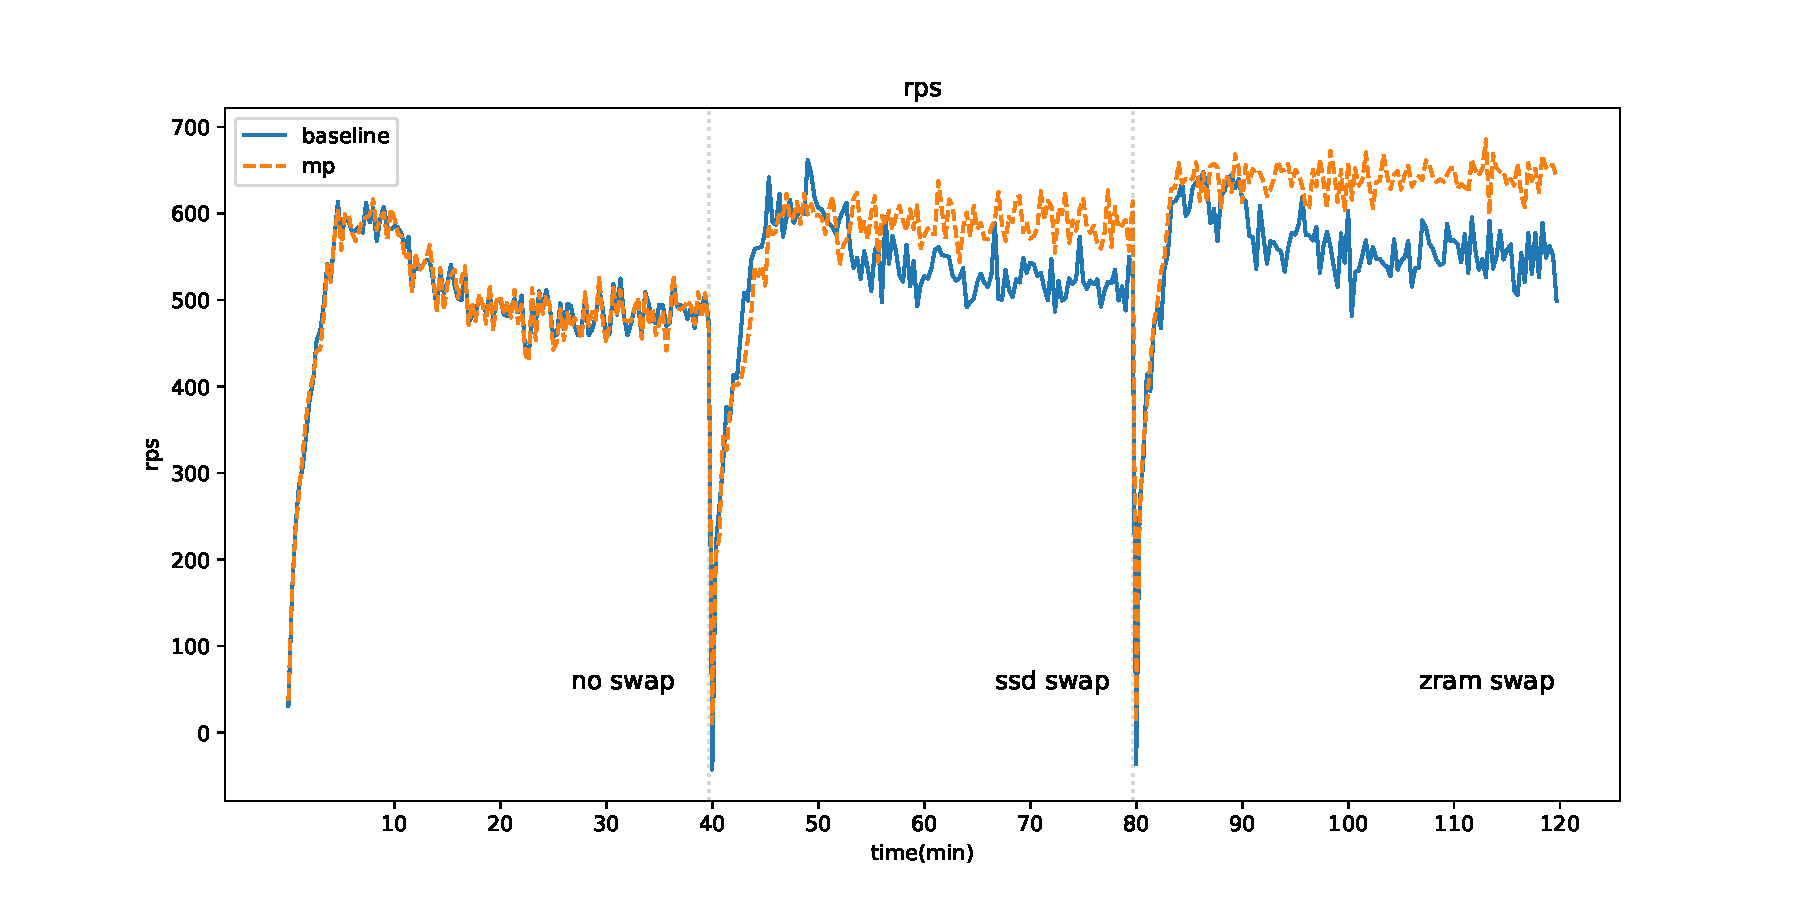
\includegraphics[width=\textwidth]{rps.pdf}
    \caption{Web Server 负载在多种场景下的 RPS 对比}
    \label{fig:rps}
\end{figure}

从内存使用角度而言,图~\ref{fig:mem}展示了不同时刻系统实际占用的内存空间。禁止 \texttt{swap} 时的占用最为紧张,一旦工作集超出物理可用范围,性能会大幅波动。SSD \texttt{swap} 能在一定程度上释放物理内存,但幅度有限;zram 则借助压缩手段使得内存占用有明显下降。若配合自适应回收算法,系统会更积极地识别低频访问页面,并在合适时机将其卸载,从而在相同负载下保持更低的物理内存占用。值得强调的是 zram 场景的差异更为显著,说明当卸载后端访问成本较低时,内核会更加大胆地进行页面回收,以换取主内存空间的可用度。

\begin{figure}[h]
    \centering
    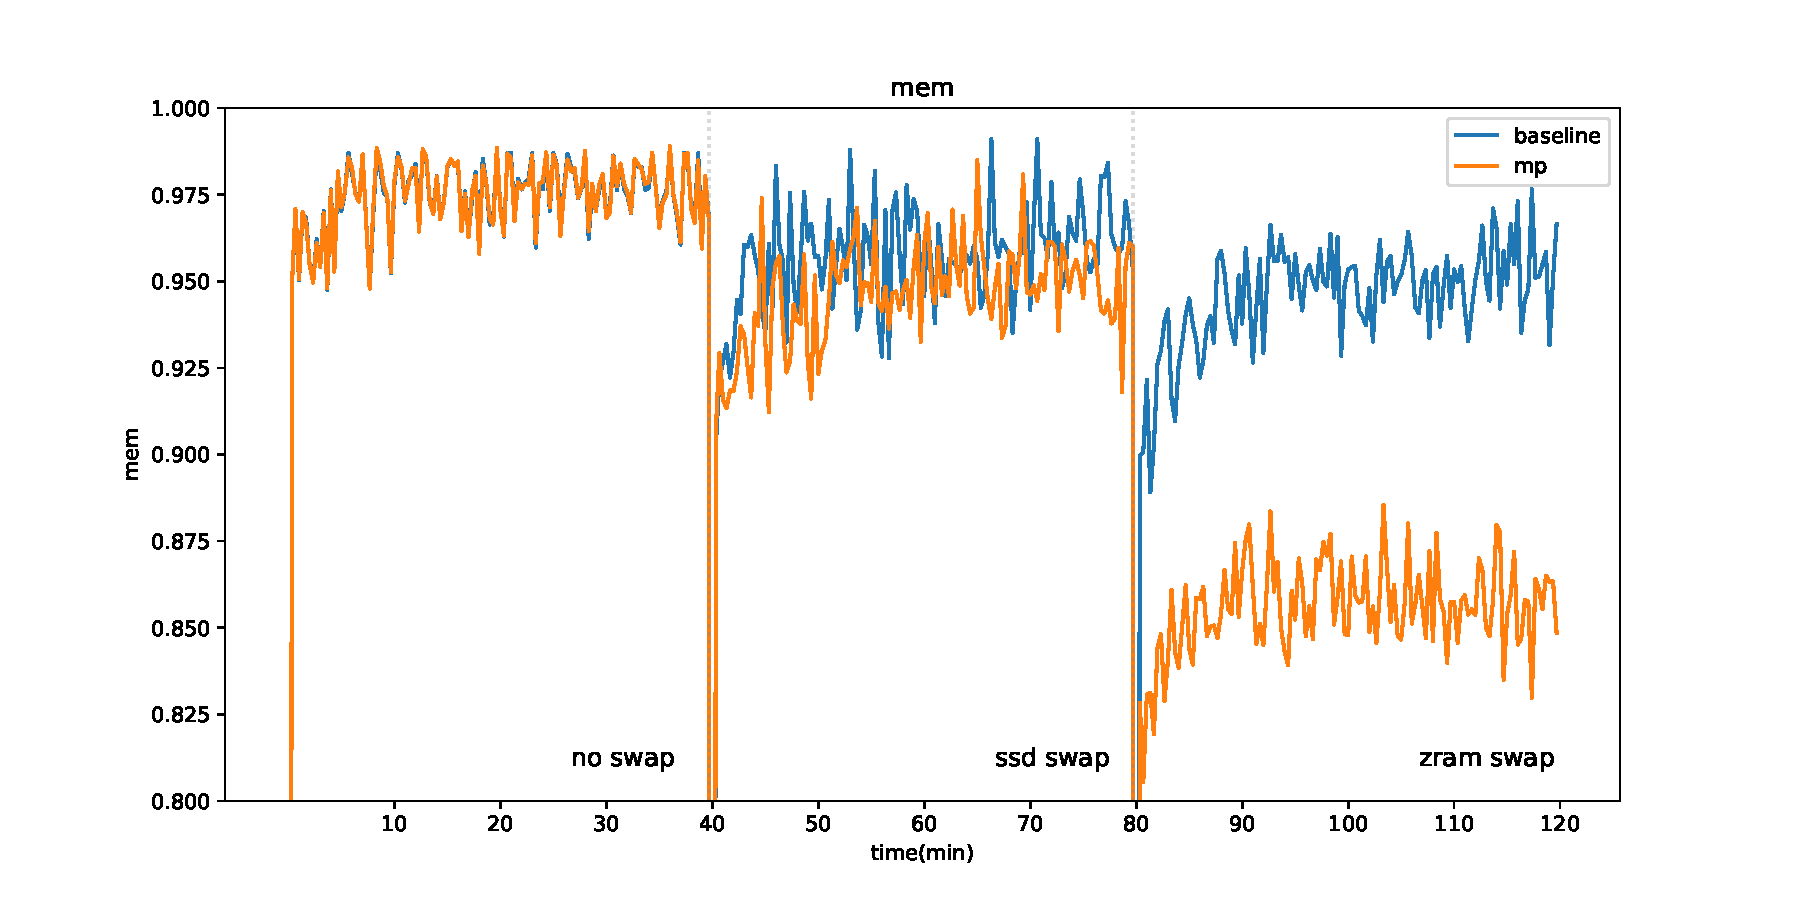
\includegraphics[width=\textwidth]{mem.pdf}
    \caption{Web Server 负载在多种场景下的内存使用对比}
    \label{fig:mem}
\end{figure}

在缺页中断次数方面,图\ref{fig:refault}显示了随着时间推移不同 \texttt{swap} 策略下的 refault 变化。zram 由于读写延迟远小于机械硬盘或常规 SSD,系统在侦测到其性能优势后往往会更积极地回收页面,一旦后续访问到已被回收的页面便会触发缺页中断,于是 zram 场景的 refault 次数偏高。表面上看这似乎意味着更多的页面换入操作,但其实际代价因为 zram 极低的访问延迟而相对有限,因此并不会对系统吞吐形成严重拖累。

\begin{figure}[h]
    \centering
    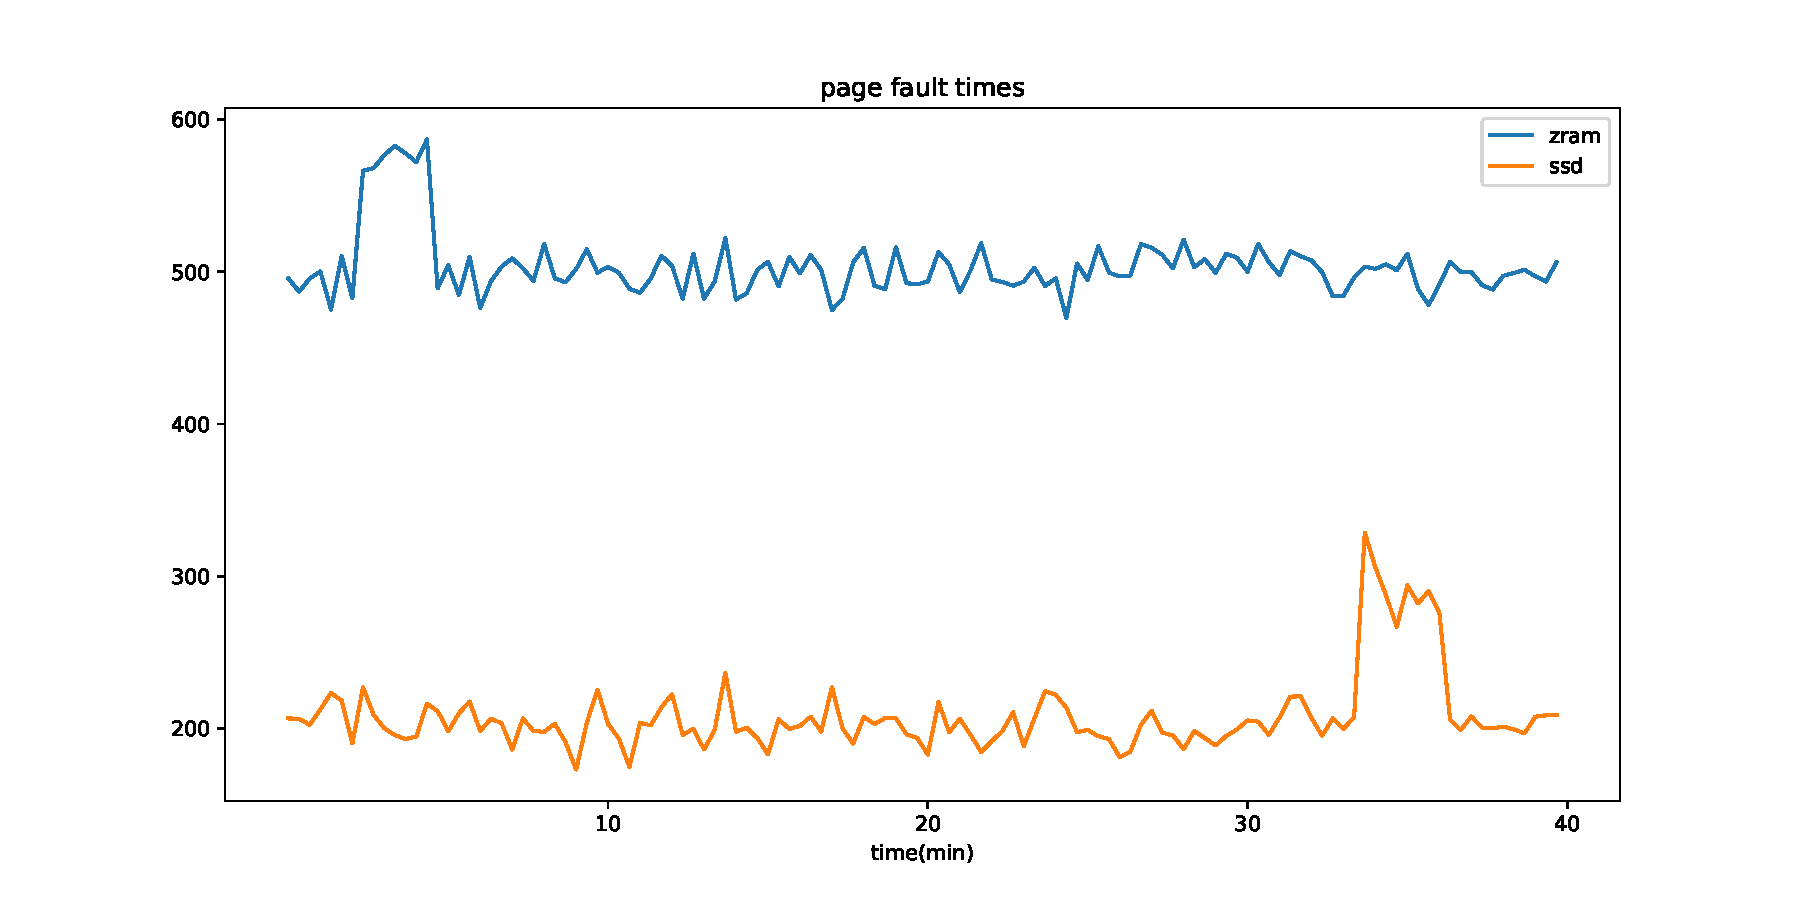
\includegraphics[width=\textwidth]{refault.pdf}
    \caption{Web Server 负载在多种场景下的缺页中断次数}
    \label{fig:refault}
\end{figure}

p90 响应时间如图~\ref{fig:p90}所示,能够比较直观地体现系统在尾部延迟上的表现。可以看到在 SSD 作为卸载后端时,由于其 I/O 性能虽优于 HDD 但依旧是一个相对独立的外部存储介质,随机小块读写性能不及压缩内存,p90 相对略高且更易抖动;而 zram 场景在高压缩比与高吞吐特性下,能将尾部延迟维持在一个更低且更稳定的水平。当结合自适应算法后,zram 场景的 p90 再度下降,说明该算法可以及时识别并淘汰不活跃页面,从而降低了频繁换入对关键请求导致的尾部延迟。

\begin{figure}[h]
    \centering
    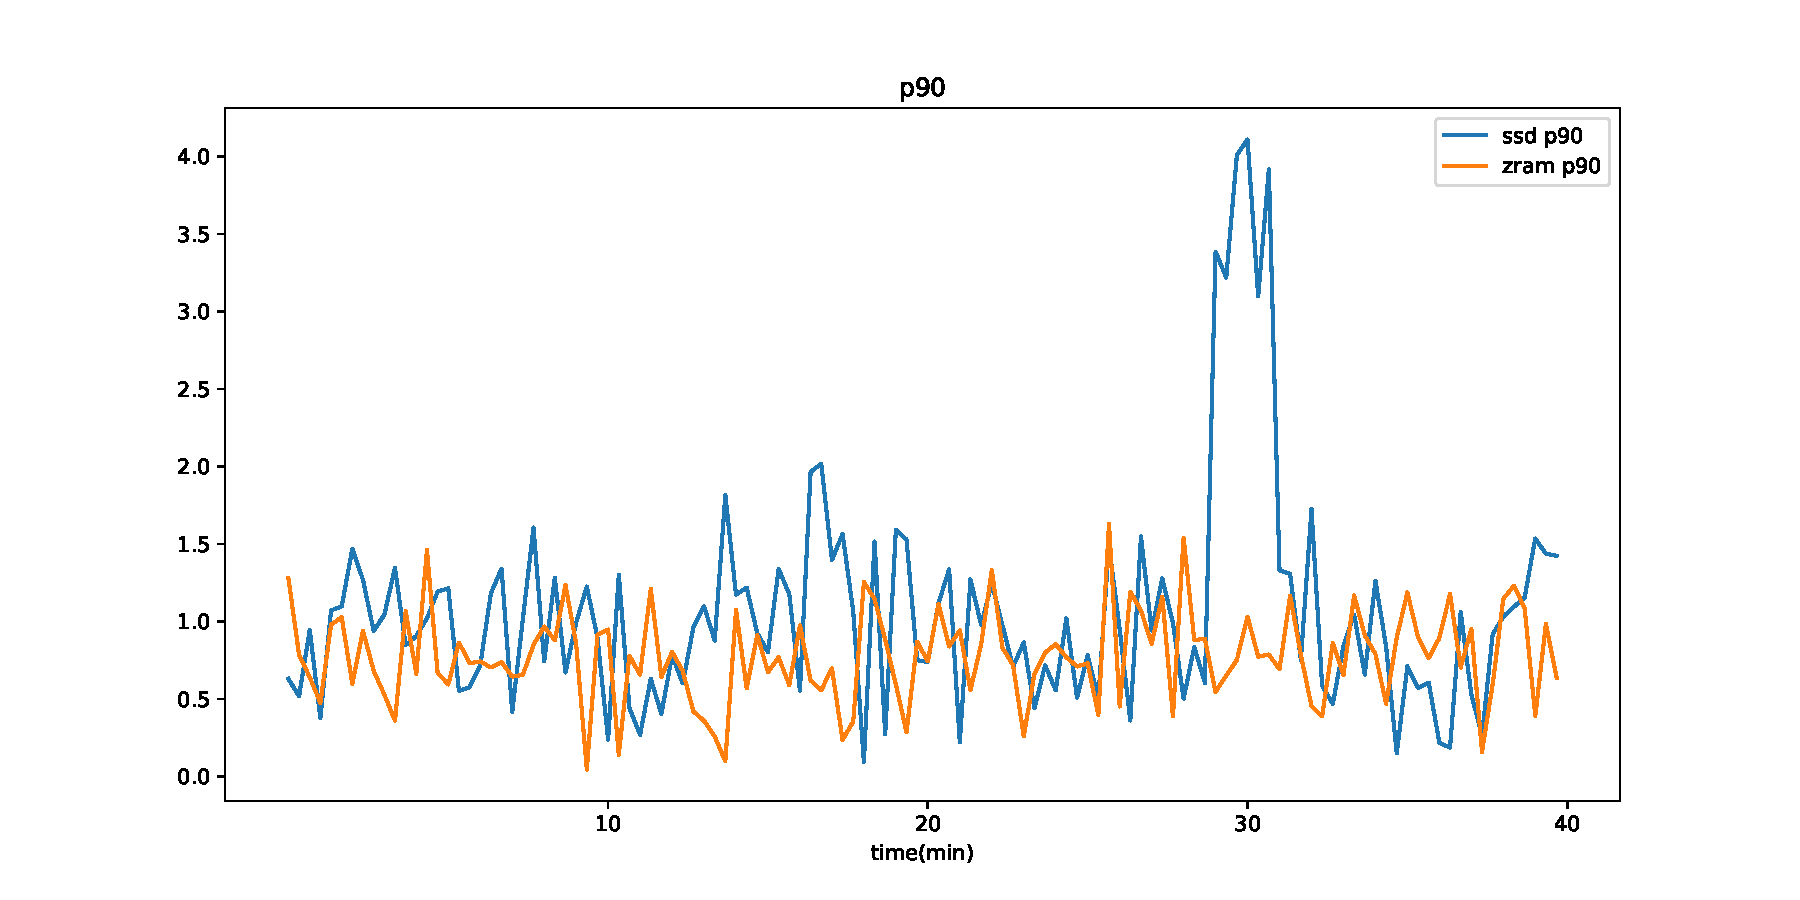
\includegraphics[width=\textwidth]{p90.pdf}
    \caption{Web Server 负载在多种场景下的 p90 响应时间对比}
    \label{fig:p90}
\end{figure}

最后,图~\ref{fig:container_memory}展示了容器化场景下的实验结果,特别关注了当 Kubernetes 或类似系统为每个 Pod 创建顶层 cgroup 并在其中运行边车容器与业务容器时,整体内存使用的变化。随着容器数量规模的增长,边车容器在日志、流量代理和监控探针等方面产生的“虚拟化税”累积效应会日益突出。本研究在容器环境中同样利用内存压力模块与自适应回收算法对边车容器和核心负载容器进行同时检测,实测表明边车容器中相当一部分页面实际上是低频或不活跃数据,卸载到高性能介质(尤其是 zram)后可有效释放物理内存,从而将更多主内存资源留给核心负载,增强了集群整体的资源利用率与稳定性。

\begin{figure}[h]
    \centering
    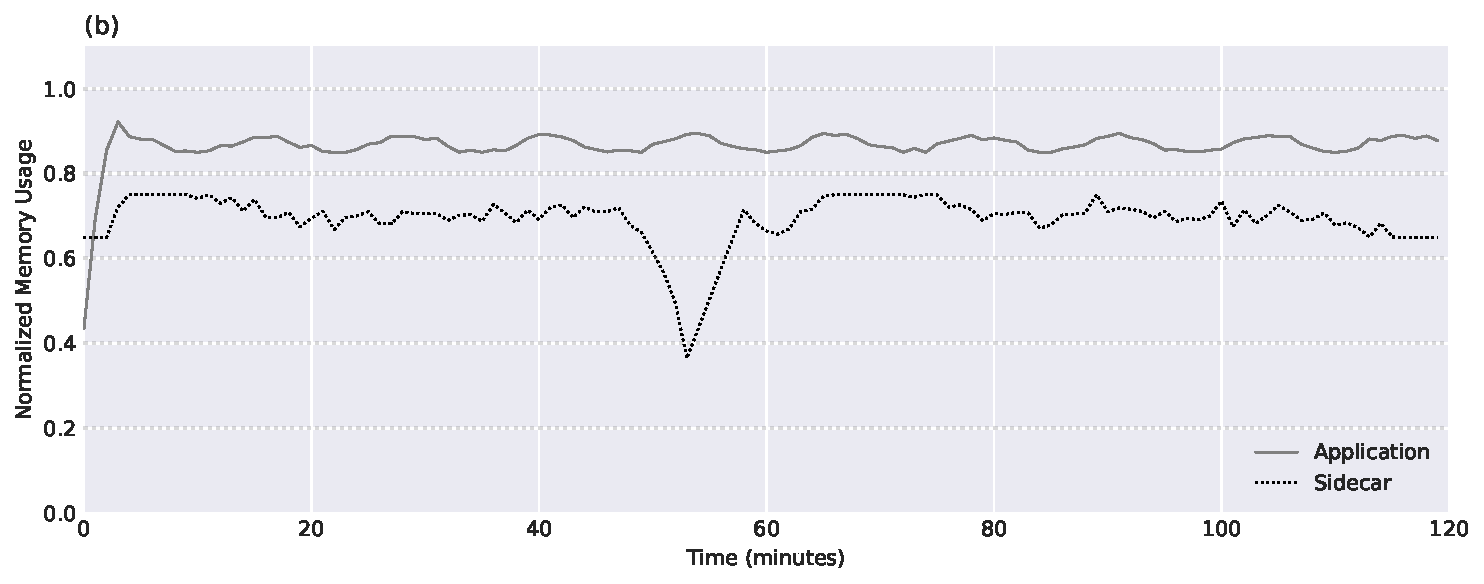
\includegraphics[width=\textwidth]{container_memory.pdf}
    \caption{容器环境下多容器运行时的内存占用}
    \label{fig:container_memory}
\end{figure}

\section{本章小结}

通过本章一系列实验,可以得出以下主要结论:首先,本文所设计的内存压力模块能够在机械硬盘、SSD 和 zram 这三种卸载后端下有效触发和量化系统的内存压力,为后续回收算法提供真实的环境支撑。其次,文件页与匿名页均衡算法在文件密集型和内存密集型负载中均展现出良好的适用性,其针对 \texttt{swappiness} 的动态调节可避免过度回收缓存文件页或引发过度的匿名页换入换出,从而在不同场景里带来显著性能增益。再次,在综合测试中,结合内存压力与自适应均衡的整体方案能够高效地释放物理内存并在高负载时保持稳定的吞吐和延迟表现,其中 zram 作为卸载后端时展现了更加出色的性能。最后,在容器化场景下,边车容器的内存占用常常在实际部署中造成可观的资源浪费,通过在内核中实施基于压力的自适应回收机制,能够大幅降低这部分“虚拟化税”,在大规模服务环境下具有突出的应用价值。上述结论为下一步在更复杂或更大规模生产环境中推广这一内存回收与卸载方案提供了重要参考依据。
